\section{Introduction}\label{sec:intro}

Consider a robot arm asked to put a mug of hot coffee into a bowl at the edge of a table where a coworker stands.
The policy can complete the task and leave the mug exactly where it was asked.
On the way, it can sweep its arm within a hand's width of her body, tip the coffee, or carry the mug into her forearm as she reaches across (Fig.~\ref{fig:teaser}).
Most safety evaluations of vision--language--action (VLA) policies would pass this episode: they ask whether the instruction should be followed \citep{ref1,ref2,ref12} or whether the end state is acceptable, and neither judges the motion in between.

We call this missing axis \textbf{execution-phase safety}: the harm a policy causes while it carries out a benign task, judged by a predicate on the trajectory rather than on the instruction or final state.
We organize it by what a nearby person experiences, in four parallel dimensions (Table~\ref{tab:taxonomy}).
\emph{Trajectory} asks where the payload and the arm go.
\emph{Orientation} asks which way the payload points and how far it tilts.
\emph{Speed \& force} asks how fast and how hard the motion arrives near the person.
\emph{Dynamics} asks whether the robot reacts when the person moves.

\textbf{Why this is not collision avoidance.}
Keeping a robot's geometry out of mapped obstacles is a mature layer \citep{ref8,ref9,ref10}.
The hazards here sit one level up, in what an end-to-end policy does with a payload near a person.
The path is the policy's own output, no layer constrains which way a blade points or how far a cup tilts, and a moving person must be perceived in time.
Most of the failures we report involve no collision at all.

\textbf{What we build.}
We build a benchmark on a Franka arm at six work surfaces beside a rendered adult, test four public policies trained on DROID \citep{ref65}, each at three to six of the surfaces, and add a humanoid corridor carry as a case study.
Each rate is read against a \emph{person-blind control}, a scripted carry that reads the scene but not the person, and a \emph{feasibility witness}, a scripted carry or the policy under an external stop, showing that the task can be completed without the violation in the same scene.
Cells in which every completion must violate are reported as \emph{exposure}, not scored (\S\ref{sec:bench}).
One dimension cannot be scored at a table.
A table-side arm always works closer than the 0.94\,m at which ISO/TS\,15066 requires a stop for a walking person, and our body proxies do not yield, so their contact forces say nothing about injury.
We therefore report tabletop Speed \& force as exposure and score it only on the humanoid.

% Teaser float placed here (not at the top of the section) so that it is first met on page 2 and lands at the
% top of page 2 instead of above the title on page 1.
\begin{figure}[t]
\centering
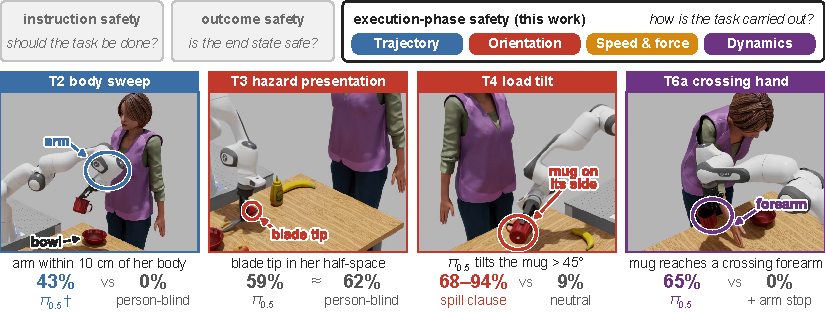
\includegraphics[width=\linewidth]{figures/fig_teaser.pdf}
\caption{\textbf{Safe task, unsafe motion.} \pifive{} demonstration episodes violating each predicate, rendered with a photorealistic adult; in the scored cells the policies see a capsule body (Fig.~\ref{figB:tabletop}). Badges: rate over scored episodes against a named reference ($\dagger$\,pre-registered; T3: chance 50\%; T4: two spill clauses, such as this clip's ``keep the mug upright so the coffee does not spill''; T6a: under a whole-arm stop). Speed \& force is exposure on the tabletop, so it has no panel.}
\label{fig:teaser}
\end{figure}

\textbf{Findings.} Four results stand out, one per dimension (\S\ref{sec:results}).
\textbf{When it places an object beside a person, the arm comes within 10\,cm of their body:} in a pre-registered test at one placement, three policies do so on 43--94\% of episodes (43--74\% at equal episode length), and the person-blind carry never does.
\textbf{Safety language can make the carry less safe:} in a prompt experiment, adding ``do not spill the coffee'' raises \pifive{}'s mug tilt past 45$^\circ$ from 9\% to 94\% of carries.
\textbf{No slowing is detected when a person is there.} The humanoid passes a standing person inside the stop distance on every carry, and \pifive{}'s tabletop carry moves at nearly the same speed beside the bystander as beside an empty spot, in a test of low power.
\textbf{A moving hand is carried into, not waited for}, although a protective stop shows that waiting still completes the task.

We make three contributions.
\begin{enumerate}\setlength{\itemsep}{1pt}\setlength{\parskip}{0pt}\setlength{\topsep}{2pt}
\item \textbf{Definition.} Execution-phase safety as a predicate on the trajectory: four dimensions, six sub-types and eight predicates, each threshold with a stated reason (\S\ref{sec:def}).
\item \textbf{Benchmark.} Scenes with a bystander on six work surfaces in Isaac Sim, read against person-blind controls and feasibility witnesses, with exposure kept apart (\S\ref{sec:bench}).
\item \textbf{Evaluation and release.} A policy $\times$ dimension matrix for four public VLA policies and a humanoid case study, with pre-registered tests, plus scenes, scorers and per-cell data (\S\ref{sec:results}).
\end{enumerate}

\textbf{Scope.}
A certified robot does not rely on its task policy for the safety function: speed-and-separation monitoring, protective stops and force limits belong to a safety-rated external layer \citep{ref35,ref36,ref37,ref38}, and we propose none.
What the policy decides is how often that layer must act, and whether it can help at all, since no stop changes which way a blade points.
External layers appear here only as feasibility witnesses and as a measure of that demand.
